\PassOptionsToPackage{unicode}{hyperref}
\documentclass[t]{beamer}

\usepackage[
  orientation=portrait,
  size=a0,
  scale=1.0,
]{beamerposter}

\usetheme{tudoposter}
\tcbuselibrary{breakable}
\usepackage{fontspec}

\usepackage{polyglossia}
\setmainlanguage{german}

\usepackage{csquotes}
\usepackage{microtype}
\usepackage{mathtools}
\usepackage{booktabs}

\usepackage[
  math-style=ISO,
  bold-style=ISO,
  nabla=upright,
  partial=upright,
]{unicode-math}
\setmathfont{Tex Gyre Pagella Math}

\usepackage[locale=DE, binary-units]{siunitx}

\usepackage{blindtext}

\usepackage{multicol}
\setlength{\columnsep}{1em}

\usepackage{graphicx}
\usepackage{ragged2e}

\usepackage{tikz}

%% this is used to create an inline bibliography
\usepackage[backend=biber, style=numeric]{biblatex}
\addbibresource{lit.bib}

\DeclareFieldFormat*{title}{\textit{#1}}
\renewcommand*{\bibfont}{\footnotesize}
\defbibenvironment{bibliography}
  {\noindent}
  {\unspace}
  {}

\renewbibmacro*{begentry}{%
  \usebeamercolor{bibliography item}%
  \color{bibliography item.fg}%
  \printtext[labelnumberwidth]{%
    \printfield{prefixnumber}%
    \printfield{labelnumber}%
  }%
  \setunit{\addnbspace}%
}
\renewcommand*{\finentrypunct}{\addperiod\space}

\newlength{\thirdtextwidth}
\setlength\thirdtextwidth{0.333333\textwidth}


\title{Datenanalyse mit IceCube Monte Carlo Daten}
\author{Maximilian Nöthe \and Kai Brügge}

\titlegraphic{%
  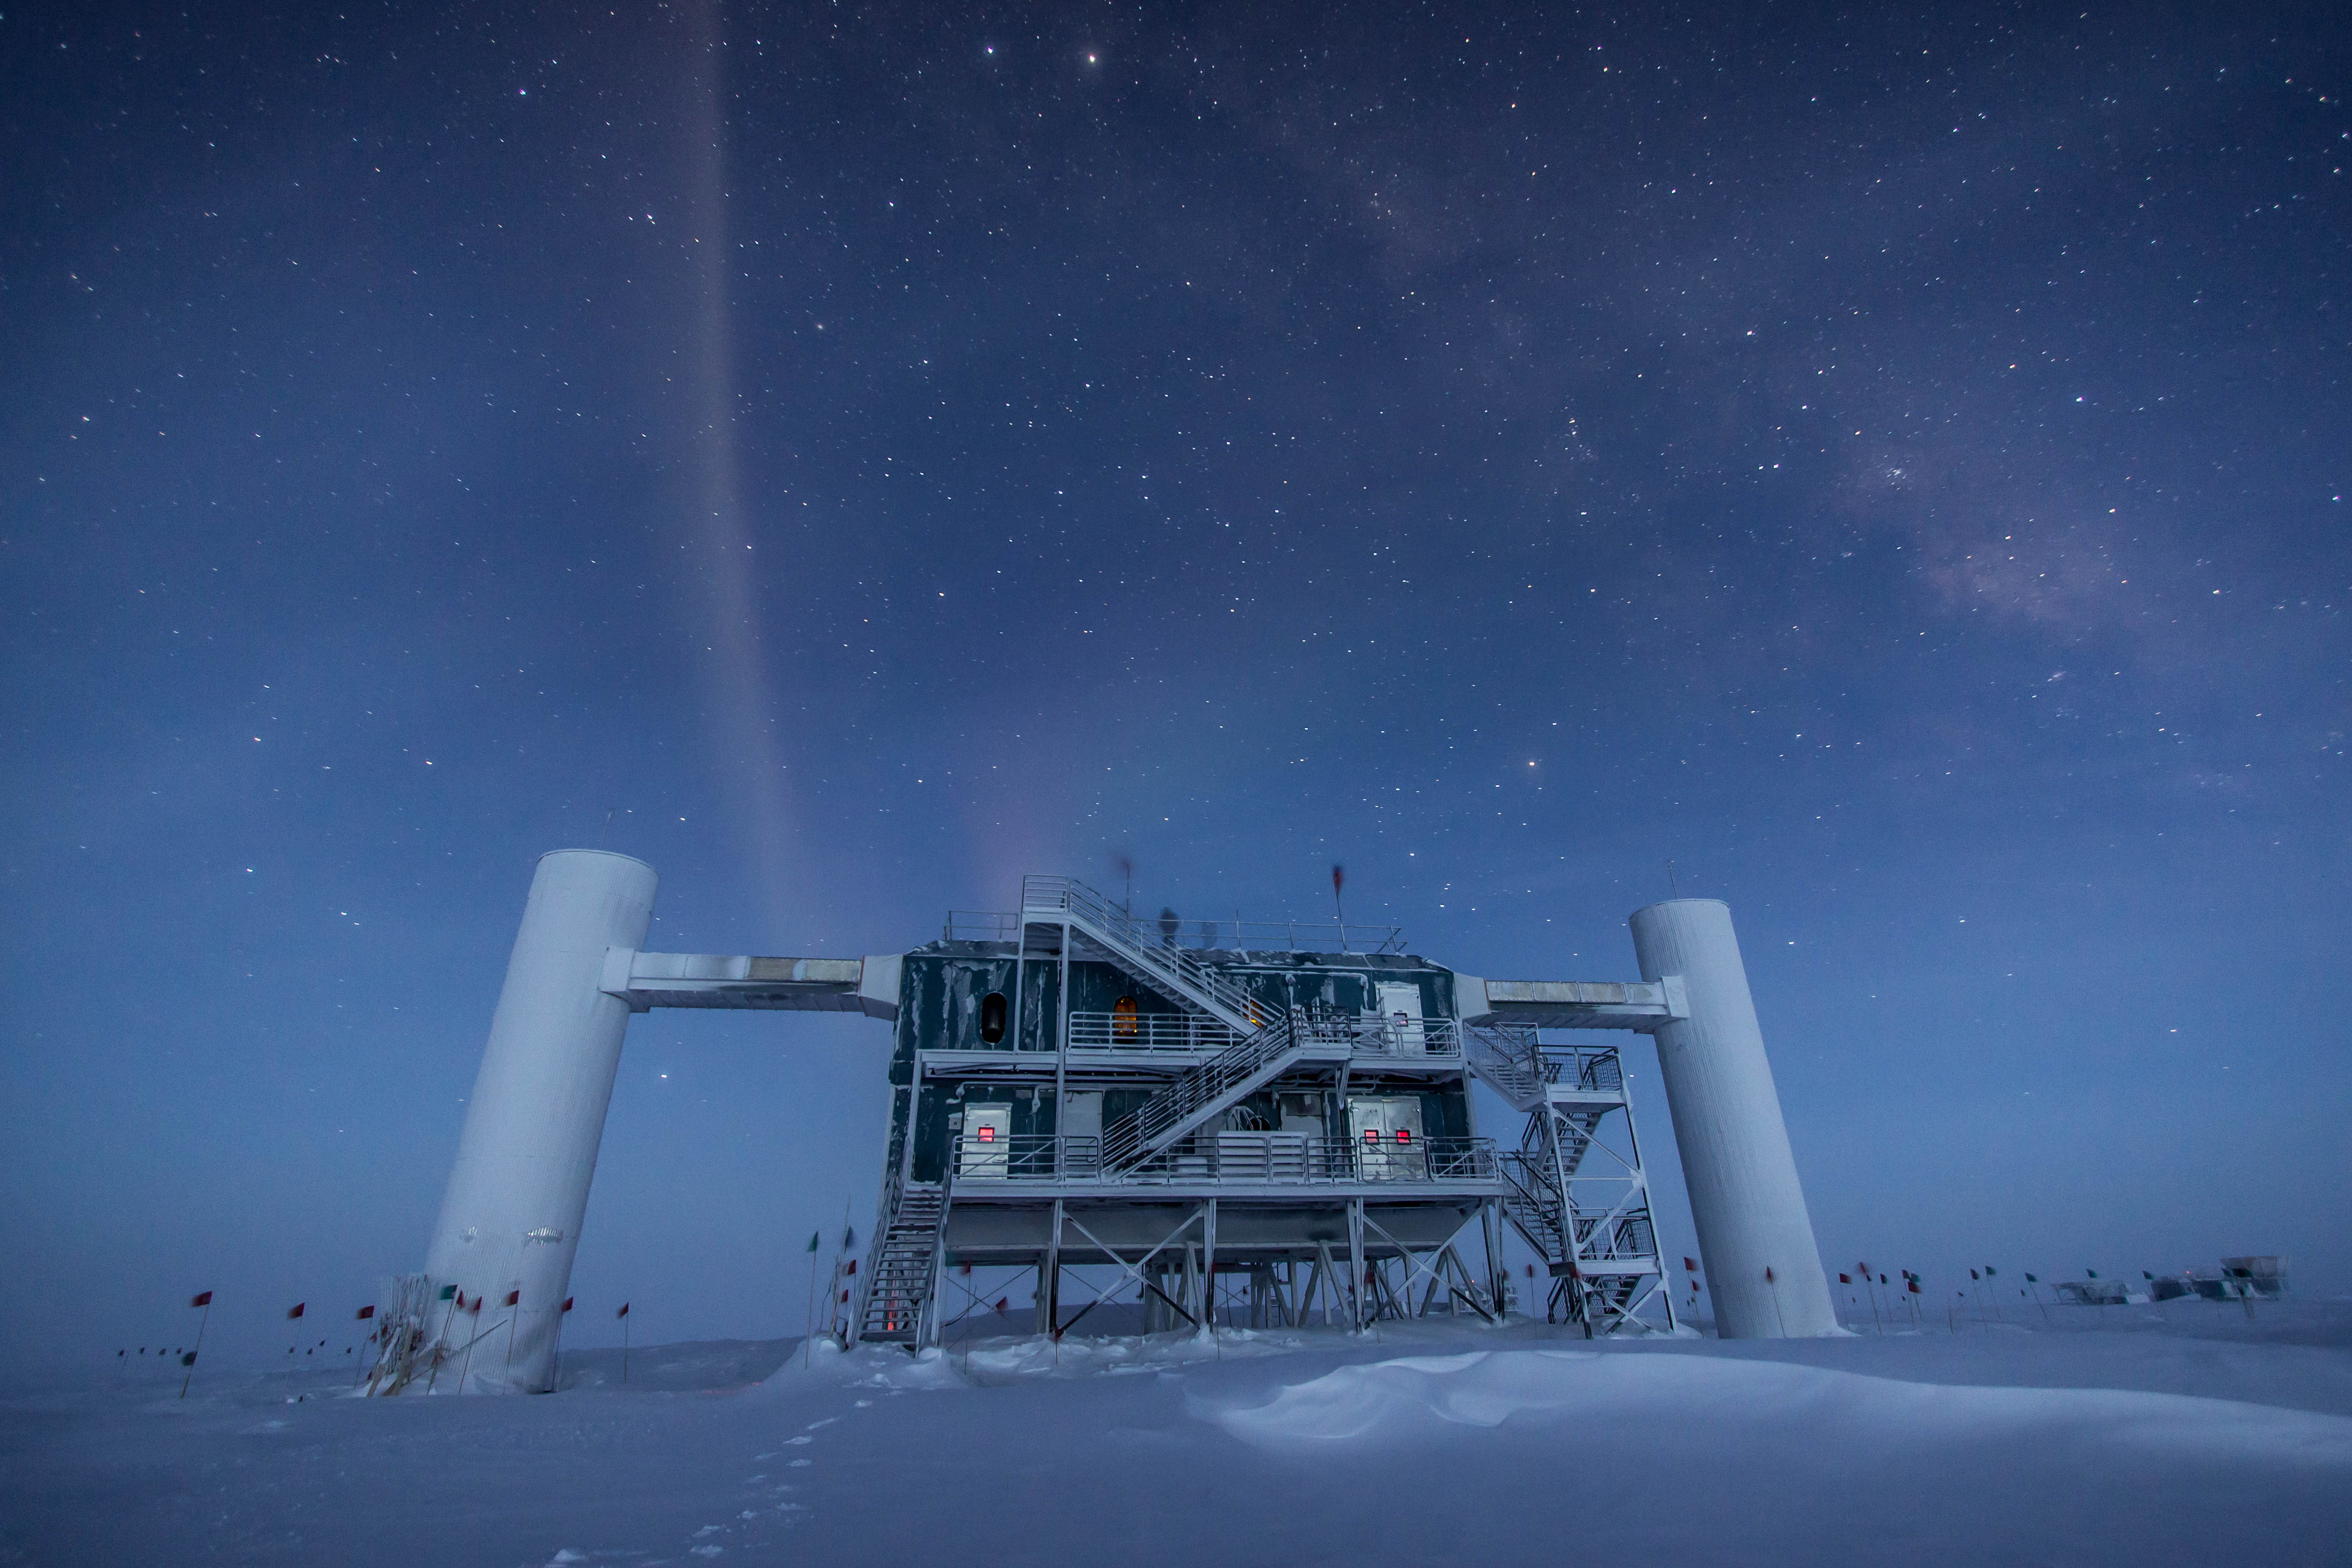
\includegraphics[width=\linewidth]{images/icecube.jpg}
}
\institute{%
  
\includegraphics[width=0.9\linewidth]{tudo.pdf}%
}

\begin{document}
  \begin{columns}[onlytextwidth]%
    \begin{column}{0.5\textwidth}%
      \begin{block}{Das IceCube Experiment}%
        \begin{columns}[onlytextwidth]%
          \begin{column}{0.48\textwidth}%
            \begin{figure}
              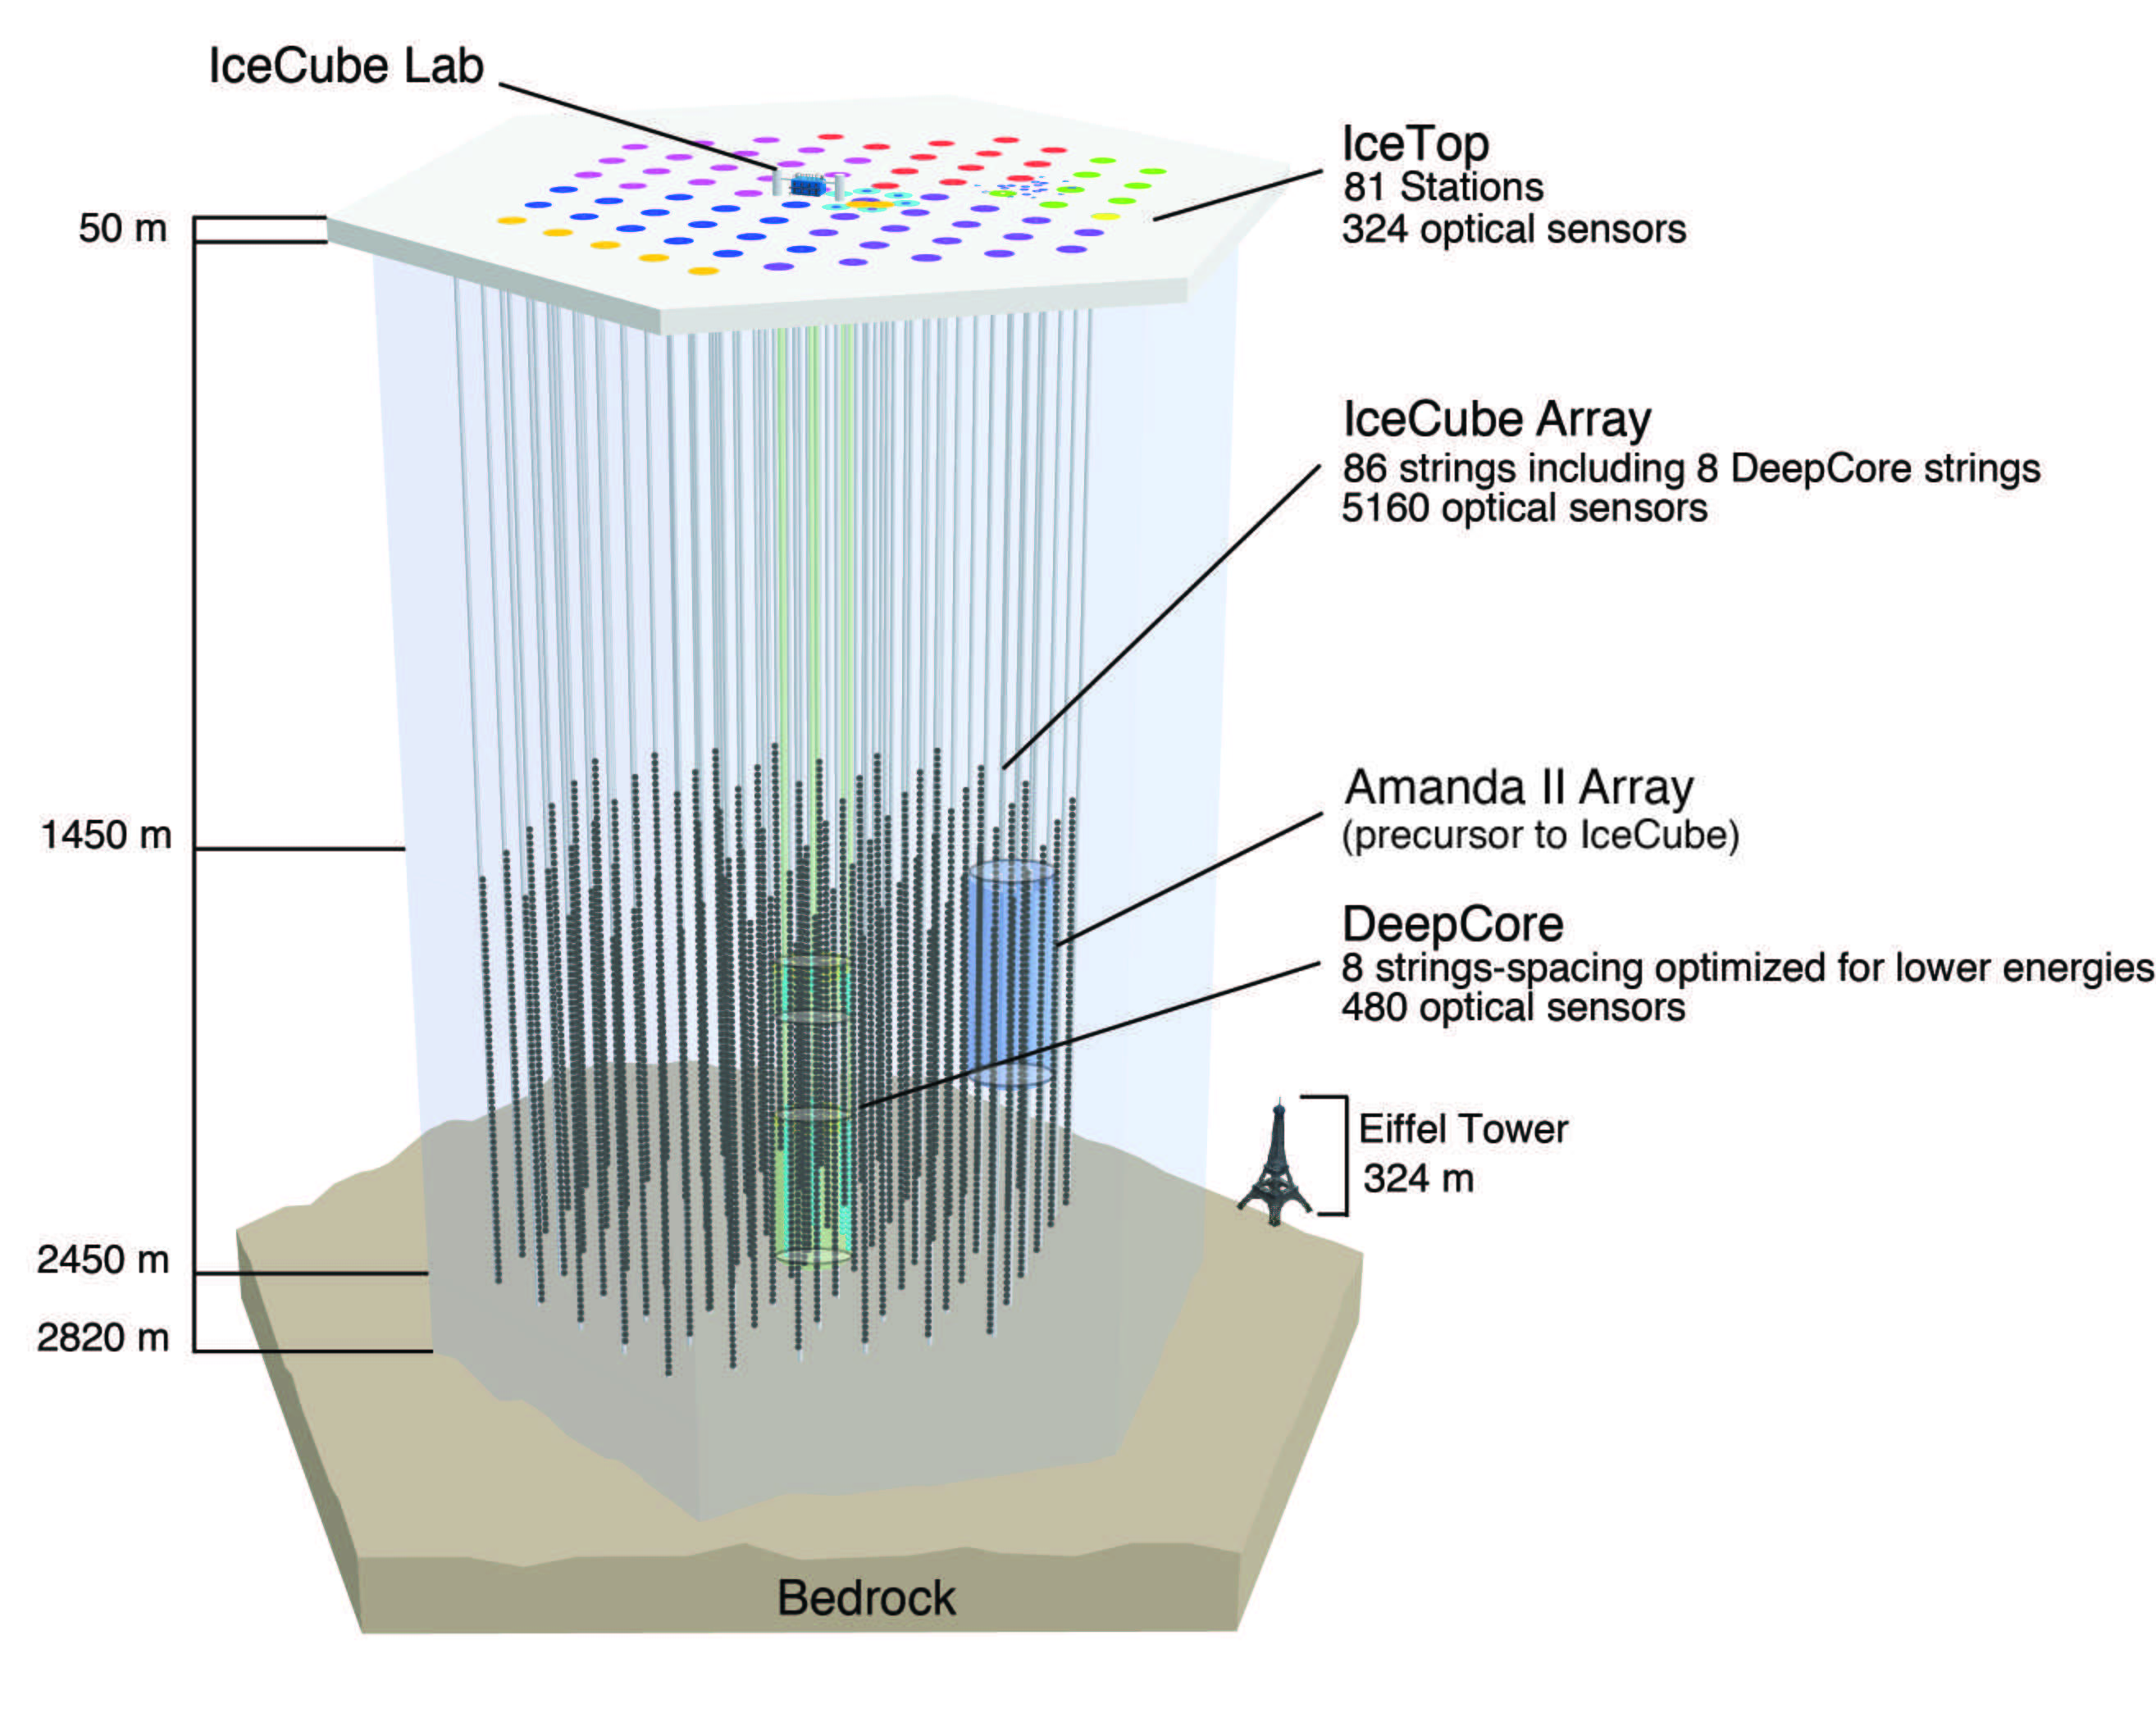
\includegraphics[width=\linewidth]{images/icecube_schema.jpg}\\
              \caption{Schematische Übersicht des IceCube Detektors~\cite{icecube_pic}.}
            \end{figure}
          \end{column}\hfill
          \begin{column}{0.48\textwidth}%
            \justifying
            Das IceCube Experiment befindet sich im Eis des geographischen Südpols.
            Das Ziel des Experiments ist das Messen von kosmischen Neutrinos.
            Hierbei stellt ein Untergrund aus atmosphärischen Myonen und Neutrinos eine
            große Herausforderung dar.

            Nachgewiesen werden Neutrinos über das Tscherenkow-Licht von Sekundärteilchen,
            die bei der Wechselwirkung der Neutrinos mit den Atomen des Eises entstehen.

            Der Detektor besteht aus insgesamt \num{5160} Photodetektoren,
            die an \num{86} einzelnen Strängen in einer Tiefe zwischen
            \SI{1450}{\meter} und \SI{2450}{\meter} im Eis eingelassen sind.

            IceCube nimmt pro Tag etwa \SI{1}{\tera\byte} Daten.
            Der erste Nachweis kosmischer Neutrinos gelang 2013~\cite{icecube_science}.
          \end{column}%
        \end{columns}%
      \end{block}%
      \begin{block}{Verwendete Software}%
        Für den Versuch wird der sogenannte \enquote{Scientific Python Stack} verwendet \cite{scipy,matplotlib,sklearn,numpy}.\par
        \begin{tikzpicture}
          \node at (0, 0) {
\includegraphics[height=2.5cm]{images/python.pdf}};
          \node at (15cm, 0.0cm) {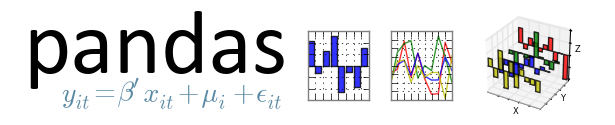
\includegraphics[height=2.5cm]{./images/pandas_logo.png}};
          \node at (0, -4cm) {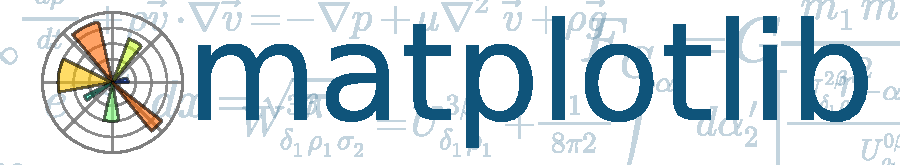
\includegraphics[height=2.5cm]{images/matplotlib.pdf}};
          \node at (15cm, -4cm) {
\includegraphics[height=3.0cm]{images/scikit-learn.pdf}};
        \end{tikzpicture}
      \end{block}
      \begin{block}{Verwendete Algorithmen}
        Zur Signal/Untergrund-Trennung werden folgende Modelle erprobt:
        \begin{description}
          \item[Gaussian Naive Bayes] Ein einfaches Modell, dass von Gaußverteilten
            Population ausgeht und ein Ereignis in die Populationen klassifiziert, für
            die die Wahrscheinlichkeit am größten ist.
          \item[Random Forest] Der Random Forest \cite{rf} besteht aus vielen Entscheidungsbäumen,
            die auf per Bootstrapping erzeugten Datensätzen gebildet werden.
            An jedem Knoten der Bäume wird nur ein zufälliges Subset aller Attribute betrachtet und davon das mit der
            stärksten Trennkraft benutzt.
            Random Forests können zusätzlich die \emph{Wichtigkeit} der Attribute für die Klassifikation
            schätzen.
          \item[AdaBoosted Trees] Ähnlich dem Random Forest sind AdaBoosted Trees \cite{adaboost}
            ebenfalls ein Ensemble-Modell aus Entscheidungsbäumen.
            Diese werden allerdings sequentiell trainiert und bei jedem neuen
            Training bekommen fehlklassifizierte Ereignisse ein erhöhtes Gewicht.
            Zur Anwendung wird ein gewichtetes Mittel über alle Bäume gebildet.
        \end{description}
      \end{block}
      \begin{block}{ROC-Kurven}
        \begin{multicols}{2}
          \begin{figure}
            \centering
            \includegraphics[width=\linewidth]{rocs_performance.pdf}
            \caption{ROC-Kurven für die drei untersuchten Modelle aus einer 10-fachen
            Kreuzvalidierung. AdaBoost und Random Forest sind ungefähr gleich stark,
          der Naive-Bayes Algorithmus ist start abgeschlagen.}
            \label{fig:name}
          \end{figure}
          \begin{center}
            \input{roc_table.tex}
          \end{center}
        \end{multicols}
      \end{block}

      \begin{block}[height=23.42cm]{Attributsauswahl}
        \begin{multicols}{2}
          \begin{figure}
            \centering
            \includegraphics[width=\linewidth]{rocs_performance_feature_selection.pdf}
            \caption{ROC-Kurven für die drei Untersuchten Modelle nach einer
              engeren Attributsauswahl. Die Auswahl erfolgte durch einen Random Forest.
              Wie erwartet, wird die Klassifikationsgüte der auf Entscheidungsbäumen basierten Modelle nicht besser.}
            \label{fig:name}
          \end{figure}
          \begin{center}
            \input{roc_table_feature_selection.tex}
          \end{center}
        \end{multicols}
      \end{block}
    \end{column}%
    \begin{column}{0.5\textwidth}%
      \begin{block}{Data-Mining}%
        \begin{multicols}{2}
          Das sehr kleine Signal-zu-Untergrund-Verhältnis von ca.\ $1:10^6$ und die
          riesigen Datenmengen des IceCube Experiments machen das
          Verwenden von Verfahren des maschinellen Lernens bzw. Data Minings nötig,
          um Signal-Ereignisse aus den Daten zu extrahieren.

          In diesem Versuch wird die Leistungsfähigkeit verschiedener Verfahren
          des maschinellen Lernens auf simulierten Daten des IceCube Experiments
          zur Klassifizierung in Signal bzw. Untergrund evaluiert.

          Signal sind hierbei alle Neutrino-Ereignisse, Untergrund sind hauptsächlich
          atmosphärische Myonen.

          Verwendet werden Methoden des überwachten maschinellen Lernens.
          Überwachte Lerner müssen auf einem Datensatz mit bekannten Wahrheiten
          \enquote{trainiert} werden und können dann auf Daten mit unbekannter
          Wahrheit angewendet werden.

          Von großer Wichtigkeit ist die Validierung der Performanz des Modells.
          Hierzu wird eine Kreuzvalidierung verwendet und mehrere Leistungskennzahlen
          ausgewertet.
        \end{multicols}
      \end{block}%

      \begin{block}{Der Datensatz}
      Der untersuchte Datensatz enthält je \num{20000} Neutrino- bzw. Untergrund-Ereignisse
      und eine hohe Anzahl von 264 bzw. 224 Attributen.

      Im ersten Schritt müssen alle Attribute verworfen werden, die nicht für
      die Klassifizierung genutzt werden können.
      Dies sind zum Beispiel:
      \begin{itemize}
        \item Monte-Carlo Wahrheiten, zum Beispiel die Energie des Primärteilchens
        \item Metadaten, wie Datum, Uhrzeit, Run-Nummer
        \item Gewichte der Ereignisse aus der Simulation
      \end{itemize}

      Hiernach bleiben 150 Attribute übrig, die sowohl für Signal, als auch für
      Untergrund vorhanden sind.
      \end{block}

      \begin{block}{Modell-Evaluierung}
        \begin{multicols}{2}
          \begin{figure}
            \centering
            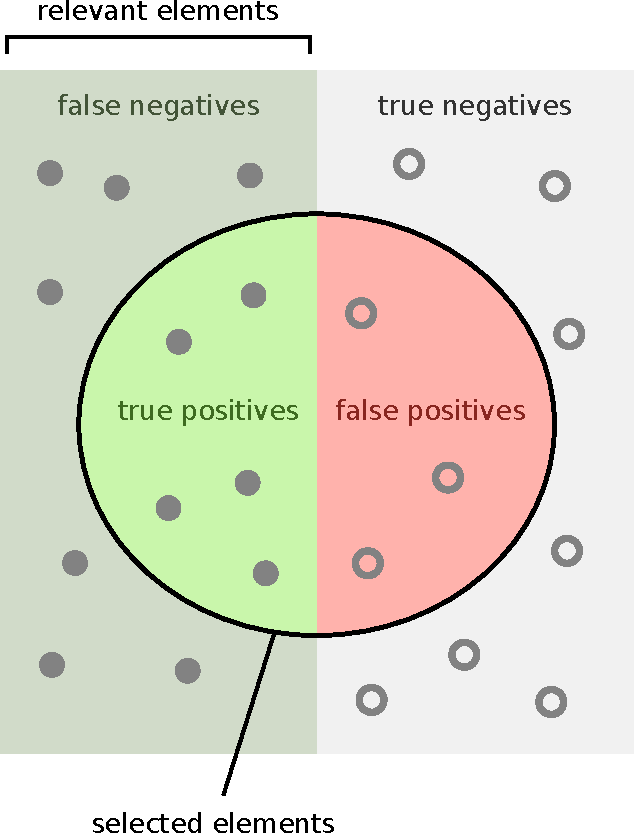
\includegraphics[width=0.9\linewidth]{images/precisionrecall-crop.pdf}
            \caption{Darstellung der Konfusionsmatrix. Links: alle Signalereignisse,
            rechts: alle Untergrundereignisse. Im Kreis befinden sich die als Signal klassifizierten Ereignisse,
            außerhalb die als Untergrund klassifizierten Ereignisse~\cite{recall_precission_pic}.}
          \end{figure}
          \columnbreak

          Ausgehend von der Konfusionsmatrix werden verschiedene Gütemaße für die maschinellen
          Lernverfahren berechnet.
          \begin{description}
            \item[Reinheit (Precision)] Anteil der wahren Signalereignisse in allen als Signal klassifizierten
              Ereignisse:
              \begin{equation}
                \mathrm{Reinheit} = \frac{\mathrm{tp}}{\mathrm{tp} + \mathrm{fp}}
              \end{equation}
            \item[Effizienz (Recall)] Anteil der als Signal klassifizierten Signalereignisse an
              allen Signalereignissen.
              \begin{equation}
                \mathrm{Effizienz} = \frac{\mathrm{tp}}{\mathrm{tp} + \mathrm{fn}}
              \end{equation}
            \item[Falsch-Positiv-Rate] Anteil der als Signal klassifizierten Untergrundereignisse
              an allen Untergrundereignisse:
              \begin{equation}
                \mathrm{fpr} = \frac{\mathrm{fp}}{\mathrm{fp} + \mathrm{tn}}
              \end{equation}
          \end{description}

          Für Modelle, die Wahrscheinlichkeitsaussagen treffen können, zum Beispiel
          ein Random Forest, sind diese Werte abhängig von der Vorhersageschwelle, ab
          der ein Ereignis einer Klasse zugewiesen wird.

          Ein Gütemaß, welches unabhängig von der Vorhersageschwelle ist, ist die Fläche
          unter dem ROC-Graphen. Im ROC-Graphen wird die Effizienz gegen die Falsch-Positiv-Rate
          aufgetragen.
          Für eine perfekte Klassifikation beträgt die Fläche unter dem ROC-Graphen~$1$.
        \end{multicols}
      \end{block}
      \begin{block}{Reinheit und Effizienz}
        \includegraphics[width=\linewidth]{precision_recall.pdf}
      \end{block}

      \begin{block}[]{Referenzen}
        \begin{multicols}{2}
          \footnotesize%
          \printbibliography%
        \end{multicols}
      \end{block}
    \end{column}%
  \end{columns}%

  % \vspace*{\fill}
\end{document}
